\documentclass[8pt,a4paper]{extarticle}

% ── Packages ──────────────────────────────────────────────────────────
\usepackage[margin=0.65in,includeheadfoot,headheight=14pt]{geometry}
\usepackage[table]{xcolor}
\usepackage{colortbl}
\usepackage{booktabs}
\usepackage{tabularx}
\usepackage{array}
\usepackage{tcolorbox}
\usepackage{tikz}
\usetikzlibrary{positioning,calc,shapes.geometric,backgrounds}
\usepackage{fontawesome5}
\usepackage{titlesec}
\usepackage{fancyhdr}
\usepackage{hyperref}
\usepackage{enumitem}
\usepackage{caption}
\usepackage{parskip}

% ── Colors ────────────────────────────────────────────────────────────
\definecolor{primary}{HTML}{1B3A5C}
\definecolor{secondary}{HTML}{2E8B8B}
\definecolor{accent}{HTML}{6B7B8D}
\definecolor{bglight}{HTML}{F0F4F8}

\hypersetup{colorlinks=true,linkcolor=primary,urlcolor=secondary,citecolor=accent}

% ── Compact sectioning ────────────────────────────────────────────────
\titleformat{\section}
  {\normalfont\Large\bfseries\color{primary}}
  {\thesection}{0.6em}{}[\vspace{-2pt}\color{primary}{\rule{\textwidth}{0.5pt}}\vspace{-4pt}]
\titlespacing{\section}{0pt}{6pt plus 1pt}{2pt plus 1pt}
\titleformat{\subsection}
  {\normalfont\normalsize\bfseries\color{secondary}}
  {\thesubsection}{0.6em}{}
\titlespacing{\subsection}{0pt}{4pt plus 1pt}{1pt plus 1pt}

\setlist[itemize]{leftmargin=*,nosep,topsep=0pt,partopsep=0pt}

% ── Header / Footer ──────────────────────────────────────────────────
\pagestyle{fancy}
\fancyhf{}
\fancyhead[L]{\color{accent}\footnotesize\textbf{NexaMarket} \textbar{} DB Schema v2.4.1}
\fancyhead[R]{\color{accent}\footnotesize\faCalendar\ \today}
\fancyfoot[C]{\color{accent}\footnotesize\thepage}
\renewcommand{\headrulewidth}{0.4pt}
\renewcommand{\headrule}{\hbox to\headwidth{\color{primary}\leaders\hrule height\headrulewidth\hfill}}

% ── tcolorbox styles ──────────────────────────────────────────────────
\tcbset{
  schemaframe/.style={
    colback=white,colframe=primary,sharp corners,boxrule=0.3pt,
    left=0.5mm,right=0.5mm,top=0.5mm,bottom=0.5mm,
    before skip=2pt,after skip=1pt
  }
}

% ── Badge helpers ─────────────────────────────────────────────────────
\newcommand{\pkbadge}{\textcolor{primary}{\faKey}~PK}
\newcommand{\fkbadge}{\textcolor{secondary}{\faKey}~FK}
\newcommand{\uqbadge}{\textcolor{accent}{\faPen}~UQ}
\newcommand{\tttype}[1]{\texttt{#1}}

\newcommand{\tableheader}[2]{\subsection{\texttt{#1} \textcolor{accent}{\textbar{} #2}}}

% ── Document ──────────────────────────────────────────────────────────
\begin{document}

% ── TITLE ─────────────────────────────────────────────────────────────
\begin{tcolorbox}[colback=primary!5,colframe=primary,sharp corners,boxrule=0.8pt,
  left=5mm,right=5mm,top=5mm,bottom=5mm]
  \centering
  {\Huge\bfseries\color{primary} NexaMarket}\\[1pt]
  {\Large\color{secondary} Database Schema Documentation}\\[2pt]
  {\footnotesize\color{accent} v2.4.1 \hspace{2em} PostgreSQL 15 \hspace{2em} \today}
\end{tcolorbox}

% ── OVERVIEW ──────────────────────────────────────────────────────────
\section{Overview}

\begin{minipage}{0.48\textwidth}
  \raggedright
  NexaMarket is a multi-tenant marketplace by \textbf{Nexa Inc.} handling customer accounts, merchant storefronts, product catalogs, order processing, payments, and inventory. All timestamps are \texttt{TIMESTAMPTZ}; soft deletes use nullable \texttt{deleted\_at} with partial unique indexes. All monetary columns store integer cents.

  \begin{tcolorbox}[colback=secondary!8,colframe=secondary!40,sharp corners,boxrule=0.3pt,
    left=3mm,right=3mm,top=1.5mm,bottom=1.5mm,before skip=3pt,after skip=0pt]
    {\footnotesize\color{primary} 6 tables \textbar{} 4 enums \textbar{} 12 FK \textbar{} 18 indexes \textbar{} \textasciitilde{}20M total rows}
  \end{tcolorbox}
\end{minipage}
\par
\begin{minipage}{0.48\textwidth}
  \centering
  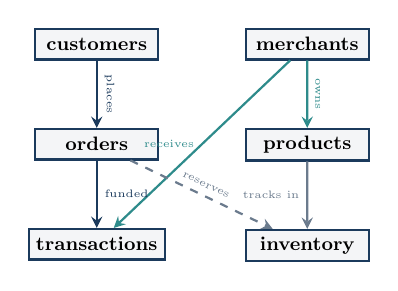
\begin{tikzpicture}[
    node distance=1.1cm and 1.4cm,
    scale=0.78, every node/.style={transform shape},
    entity/.style={rectangle,draw=primary,fill=primary!5,thick,
      minimum width=2cm,minimum height=0.5cm,font=\small\bfseries,align=center},
    every path/.style={->,>=stealth,thick}
  ]
    \node[entity] (cust)   {customers};
    \node[entity] (merch)  [right=of cust]   {merchants};
    \node[entity] (prod)   [below=of merch]  {products};
    \node[entity] (orders) [below=of cust]   {orders};
    \node[entity] (txn)    [below=of orders] {transactions};
    \node[entity] (inv)    [below=of prod]   {inventory};

    \draw[primary]   (cust)  -- node[above,sloped,font=\tiny\color{accent}] {places}   (orders);
    \draw[secondary] (merch) -- node[above,sloped,font=\tiny\color{accent}] {owns}     (prod);
    \draw[secondary] (merch) -- node[left,font=\tiny\color{accent}]        {receives}  (txn);
    \draw[primary]   (orders)-- node[right,font=\tiny\color{accent}]        {funded}    (txn);
    \draw[accent]    (prod)  -- node[left,font=\tiny\color{accent}]         {tracks in} (inv);
    \draw[accent,dashed] (orders) -- node[above,sloped,font=\tiny\color{accent}] {reserves} (inv);
  \end{tikzpicture}
  \vspace{-3pt}
  \captionof{figure}{\footnotesize\color{accent}Dashed link via \texttt{order\_items}.}
\end{minipage}
\par

% ── TABLE DEFINITIONS ─────────────────────────────────────────────────
\section{Table Definitions}

% --- customers ---
\tableheader{customers}{\textasciitilde{}2.1M rows}
\begin{tcolorbox}[schemaframe]
  \renewcommand{\arraystretch}{1.05}
  \begin{tabularx}{\linewidth}{p{2cm} p{1.6cm} X p{2cm}}
    \toprule
    \rowcolor{primary!10}\textbf{Column} & \textbf{Type} & \textbf{Constraints / Notes} \\
    \midrule
    id              & \tttype{BIGSERIAL}   & \pkbadge\ surrogate key. \\
    external\_id    & \tttype{UUID}        & \uqbadge\ API identifier. \\
    email           & \tttype{VARCHAR(255)}& \uqbadge\ Login; UNIQUE WHERE deleted\_at IS NULL. \\
    full\_name      & \tttype{VARCHAR(150)}& Display name. \\
    password\_hash  & \tttype{TEXT}        & bcrypt/argon2 digest. \\
    phone           & \tttype{VARCHAR(20)} & E.164, nullable; indexed. \\
    default\_currency& \tttype{CHAR(3)}    & Default \texttt{`USD'}. \\
    email\_verified\_at&\tttype{TIMESTAMPTZ}&NULL until confirmed. \\
    created\_at     & \tttype{TIMESTAMPTZ} & Default \texttt{now()}; indexed DESC. \\
    updated\_at     & \tttype{TIMESTAMPTZ} & Auto-updated. \\
    deleted\_at     & \tttype{TIMESTAMPTZ} & Soft-delete, nullable. \\
    \bottomrule
  \end{tabularx}
\end{tcolorbox}

% --- merchants ---
\tableheader{merchants}{\textasciitilde{}48K rows}
\begin{tcolorbox}[schemaframe]
  \renewcommand{\arraystretch}{1.05}
  \begin{tabularx}{\linewidth}{p{2cm} p{1.6cm} X p{2cm}}
    \toprule
    \rowcolor{primary!10}\textbf{Column} & \textbf{Type} & \textbf{Constraints / Notes} \\
    \midrule
    id                 & \tttype{BIGSERIAL}   & \pkbadge\ surrogate key. \\
    external\_id       & \tttype{UUID}        & \uqbadge\ Public storefront ID. \\
    store\_name        & \tttype{VARCHAR(200)}& \uqbadge\ Display name. \\
    slug               & \tttype{VARCHAR(200)}& \uqbadge\ URL-safe; UNIQUE WHERE deleted\_at IS NULL. \\
    owner\_email       & \tttype{VARCHAR(255)}& \uqbadge\ Contact / login. \\
    payout\_method     & \tttype{VARCHAR(30)} & stripe \textbar{} wise \textbar{} bank\_transfer. \\
    payout\_destination& \tttype{VARCHAR(255)}& Stripe acct ID or IBAN. \\
    commission\_bps    & \tttype{SMALLINT}    & Default 500 (5.00\%). \\
    status             & \tttype{VARCHAR(20)} & pending \textbar{} active \textbar{} suspended \textbar{} closed. \\
    created\_at        & \tttype{TIMESTAMPTZ} & Default \texttt{now()}; indexed. \\
    updated\_at        & \tttype{TIMESTAMPTZ} & Auto-updated. \\
    deleted\_at        & \tttype{TIMESTAMPTZ} & Soft-delete, nullable. \\
    \bottomrule
  \end{tabularx}
\end{tcolorbox}

% --- products ---
\tableheader{products}{\textasciitilde{}1.9M rows}
\begin{tcolorbox}[schemaframe]
  \renewcommand{\arraystretch}{1.05}
  \begin{tabularx}{\linewidth}{p{2cm} p{1.6cm} X p{2cm}}
    \toprule
    \rowcolor{primary!10}\textbf{Column} & \textbf{Type} & \textbf{Constraints / Notes} \\
    \midrule
    id               & \tttype{BIGSERIAL}   & \pkbadge\ surrogate key. \\
    merchant\_id     & \tttype{BIGINT}      & \fkbadge\ FK \textrightarrow{} merchants.id; indexed. \\
    external\_id     & \tttype{UUID}        & \uqbadge\ Public identifier. \\
    title            & \tttype{VARCHAR(300)}& Indexed; GIN trigram (pg\_trgm) for search. \\
    description      & \tttype{TEXT}        & Markdown body. \\
    category         & \tttype{VARCHAR(80)} & Indexed; electronics \textbar{} fashion \textbar{} home \textbar{} … \\
    base\_price\_cents& \tttype{BIGINT}     & Smallest currency unit. \\
    currency         & \tttype{CHAR(3)}     & Default \texttt{`USD'}. \\
    is\_digital      & \tttype{BOOLEAN}     & Default FALSE. \\
    tags             & \tttype{TEXT[]}      & PG array for search. \\
    created\_at      & \tttype{TIMESTAMPTZ} & Default \texttt{now()}. \\
    updated\_at      & \tttype{TIMESTAMPTZ} & Auto-updated. \\
    deleted\_at      & \tttype{TIMESTAMPTZ} & Soft-delete, nullable. \\
    \bottomrule
  \end{tabularx}
\end{tcolorbox}

% --- inventory ---
\tableheader{inventory}{\textasciitilde{}4.3M rows}
\begin{tcolorbox}[schemaframe]
  \renewcommand{\arraystretch}{1.05}
  \begin{tabularx}{\linewidth}{p{2cm} p{1.6cm} X p{2cm}}
    \toprule
    \rowcolor{primary!10}\textbf{Column} & \textbf{Type} & \textbf{Constraints / Notes} \\
    \midrule
    id                  & \tttype{BIGSERIAL}   & \pkbadge\ surrogate key. \\
    product\_id         & \tttype{BIGINT}      & \fkbadge\ FK \textrightarrow{} products.id; CASCADE. \\
    sku                 & \tttype{VARCHAR(64)} & \uqbadge\ Merchant-defined. \\
    variant\_label      & \tttype{VARCHAR(200)}& e.g.\ \texttt{`Size~L~/~Blue'}. \\
    quantity\_available & \tttype{INTEGER}     & Default 0; CHECK >= 0. \\
    quantity\_reserved  & \tttype{INTEGER}     & Pending-order hold; CHECK >= 0. \\
    warehouse\_location & \tttype{VARCHAR(100)}& Bin ref, nullable. \\
    low\_stock\_threshold& \tttype{INTEGER}    & Default 5. \\
    created\_at         & \tttype{TIMESTAMPTZ} & Default \texttt{now()}. \\
    updated\_at         & \tttype{TIMESTAMPTZ} & Auto-updated. \\
    \bottomrule
  \end{tabularx}
\end{tcolorbox}

% --- orders ---
\tableheader{orders}{\textasciitilde{}6.1M rows}
\begin{tcolorbox}[schemaframe]
  \renewcommand{\arraystretch}{1.05}
  \begin{tabularx}{\linewidth}{p{2cm} p{1.6cm} X p{2cm}}
    \toprule
    \rowcolor{primary!10}\textbf{Column} & \textbf{Type} & \textbf{Constraints / Notes} \\
    \midrule
    id                  & \tttype{BIGSERIAL}   & \pkbadge\ surrogate key. \\
    customer\_id        & \tttype{BIGINT}      & \fkbadge\ FK \textrightarrow{} customers.id; RESTRICT. \\
    external\_id        & \tttype{UUID}        & \uqbadge\ Customer-facing order \#. \\
    status              & \tttype{VARCHAR(20)} & pending \textbar{} confirmed \textbar{} shipped \textbar{} delivered \textbar{} cancelled; indexed (partial WHERE pending). \\
    subtotal\_cents     & \tttype{BIGINT}      & Line items sum. \\
    tax\_cents          & \tttype{BIGINT}      & Default 0. \\
    shipping\_cents     & \tttype{BIGINT}      & Default 0. \\
    total\_cents        & \tttype{BIGINT}      & subtotal + tax + shipping. \\
    currency            & \tttype{CHAR(3)}     & Default \texttt{`USD'}. \\
    shipping\_address\_id& \tttype{BIGINT}     & \fkbadge\ FK \textrightarrow{} addresses.id; SET NULL. \\
    placed\_at          & \tttype{TIMESTAMPTZ} & Default \texttt{now()}; indexed DESC. \\
    updated\_at         & \tttype{TIMESTAMPTZ} & Auto-updated. \\
    \bottomrule
  \end{tabularx}
\end{tcolorbox}

% --- transactions ---
\tableheader{transactions}{\textasciitilde{}5.9M rows}
\begin{tcolorbox}[schemaframe]
  \renewcommand{\arraystretch}{1.05}
  \begin{tabularx}{\linewidth}{p{2cm} p{1.6cm} X p{2cm}}
    \toprule
    \rowcolor{primary!10}\textbf{Column} & \textbf{Type} & \textbf{Constraints / Notes} \\
    \midrule
    id                   & \tttype{BIGSERIAL}   & \pkbadge\ surrogate key. \\
    order\_id            & \tttype{BIGINT}      & \fkbadge, \uqbadge\ FK \textrightarrow{} orders.id (1:1); RESTRICT. \\
    merchant\_id         & \tttype{BIGINT}      & \fkbadge\ FK \textrightarrow{} merchants.id; RESTRICT. \\
    external\_id         & \tttype{UUID}        & \uqbadge\ Payment reference. \\
    provider             & \tttype{VARCHAR(30)} & stripe \textbar{} wise \textbar{} paypal. \\
    provider\_txn\_id    & \tttype{VARCHAR(255)}& \uqbadge\ Gateway ref; nullable; UNIQUE WHERE NOT NULL. \\
    amount\_cents        & \tttype{BIGINT}      & Total charged. \\
    platform\_fee\_cents & \tttype{BIGINT}      & Nexa cut. \\
    merchant\_payout\_cents&\tttype{BIGINT}    & amount minus platform\_fee. \\
    currency             & \tttype{CHAR(3)}     & Default \texttt{`USD'}. \\
    status               & \tttype{VARCHAR(20)} & pending \textbar{} authorized \textbar{} captured \textbar{} refunded \textbar{} failed; indexed (partial WHERE pending). \\
    captured\_at         & \tttype{TIMESTAMPTZ} & Populated on capture. \\
    created\_at          & \tttype{TIMESTAMPTZ} & Default \texttt{now()}; indexed DESC. \\
    \bottomrule
  \end{tabularx}
\end{tcolorbox}

% ── ENUMS + FK ────────────────────────────────────────────────────────
\section{Enumerated Types \& Foreign Keys}

\begin{minipage}{0.48\textwidth}
  \begin{tcolorbox}[colback=white,colframe=secondary!50,sharp corners,boxrule=0.3pt,
    left=2mm,right=2mm,top=1.5mm,bottom=1.5mm,before skip=0pt,after skip=1pt]
    {\fontsize{7}{9}\selectfont\color{primary}\textbf{order\_status} \textbar{} \texttt{pending, confirmed, shipped, delivered, cancelled}}
  \end{tcolorbox}
  \begin{tcolorbox}[colback=white,colframe=secondary!50,sharp corners,boxrule=0.3pt,
    left=2mm,right=2mm,top=1.5mm,bottom=1.5mm,before skip=0pt,after skip=1pt]
    {\fontsize{7}{9}\selectfont\color{primary}\textbf{merchant\_status} \textbar{} \texttt{pending, active, suspended, closed}}
  \end{tcolorbox}
  \begin{tcolorbox}[colback=white,colframe=secondary!50,sharp corners,boxrule=0.3pt,
    left=2mm,right=2mm,top=1.5mm,bottom=1.5mm,before skip=0pt,after skip=1pt]
    {\fontsize{7}{9}\selectfont\color{primary}\textbf{payout\_method} \textbar{} \texttt{stripe, wise, bank\_transfer} \hspace{1em} \textbf{txn\_status} \textbar{} \texttt{pending, authorized, captured, refunded, failed}}
  \end{tcolorbox}
\end{minipage}
\par
\begin{minipage}{0.48\textwidth}
  \begin{tcolorbox}[schemaframe]
    \renewcommand{\arraystretch}{1.1}
    \begin{tabularx}{\linewidth}{p{2.3cm} p{2.5cm} X}
      \toprule
      \rowcolor{primary!10}\textbf{Child} & \textbf{Column} & \textbf{Parent (On Delete)} \\
      \midrule
      products     & merchant\_id          & merchants.id (CASCADE) \\
      inventory    & product\_id           & products.id (CASCADE) \\
      orders       & customer\_id          & customers.id (RESTRICT) \\
      orders       & shipping\_address\_id & addresses.id (SET NULL) \\
      transactions & order\_id             & orders.id (RESTRICT) \\
      transactions & merchant\_id          & merchants.id (RESTRICT) \\
      \bottomrule
    \end{tabularx}
  \end{tcolorbox}
\end{minipage}
\par

% ── SAMPLE QUERIES ────────────────────────────────────────────────────
\section{Representative Queries}

\begin{minipage}{0.48\textwidth}
  \begin{tcolorbox}[colback=bglight,colframe=accent!40,sharp corners,boxrule=0.3pt,
    left=2mm,right=2mm,top=1.5mm,bottom=1.5mm,before skip=1pt,after skip=0pt]
    {\fontsize{6.5}{8}\selectfont\color{primary}\textbf{Active listings}}\\[0.5pt]
    {\fontsize{5.5}{7}\selectfont\ttfamily
      SELECT m.store\_name, p.title, p.base\_price\_cents,\\
      \quad i.quantity\_available\\
      \quad FROM products p\\
      \quad JOIN merchants m ON m.id=p.merchant\_id\\
      \quad JOIN inventory i ON i.product\_id=p.id\\
      \quad WHERE p.deleted\_at IS NULL\\
      \qquad AND m.status=`active'\\
      \qquad AND i.quantity\_available>0\\
      \quad ORDER BY p.created\_at DESC LIMIT 50;
    }
  \end{tcolorbox}
\end{minipage}
\par
\begin{minipage}{0.48\textwidth}
  \begin{tcolorbox}[colback=bglight,colframe=accent!40,sharp corners,boxrule=0.3pt,
    left=2mm,right=2mm,top=1.5mm,bottom=1.5mm,before skip=1pt,after skip=0pt]
    {\fontsize{6.5}{8}\selectfont\color{primary}\textbf{Daily revenue (30d)}}\\[0.5pt]
    {\fontsize{5.5}{7}\selectfont\ttfamily
      SELECT DATE(captured\_at) AS day,\\
      \quad COUNT(*) AS txn\_count,\\
      \quad SUM(amount\_cents) AS gross,\\
      \quad SUM(platform\_fee\_cents) AS revenue\\
      \quad FROM transactions\\
      \quad WHERE status=`captured'\\
      \qquad AND captured\_at>=now()-INTERVAL `30d'\\
      \quad GROUP BY day ORDER BY day DESC;
    }
  \end{tcolorbox}
\end{minipage}
\par

\vspace{2pt}

\begin{minipage}{0.48\textwidth}
  \begin{tcolorbox}[colback=bglight,colframe=accent!40,sharp corners,boxrule=0.3pt,
    left=2mm,right=2mm,top=1.5mm,bottom=1.5mm,before skip=1pt,after skip=0pt]
    {\fontsize{6.5}{8}\selectfont\color{primary}\textbf{Low-stock alert}}\\[0.5pt]
    {\fontsize{5.5}{7}\selectfont\ttfamily
      SELECT p.title, i.sku,\\
      \quad i.quantity\_available, i.low\_stock\_threshold\\
      \quad FROM inventory i\\
      \quad JOIN products p ON p.id=i.product\_id\\
      \quad WHERE i.quantity\_available\\
      \qquad <=i.low\_stock\_threshold\\
      \qquad AND p.deleted\_at IS NULL\\
      \quad ORDER BY i.quantity\_available ASC;
    }
  \end{tcolorbox}
\end{minipage}
\par
\begin{minipage}{0.48\textwidth}
  \begin{tcolorbox}[colback=secondary!6,colframe=secondary!50,sharp corners,boxrule=0.4pt,
    left=2mm,right=2mm,top=1.5mm,bottom=1.5mm,before skip=1pt,after skip=0pt]
    {\fontsize{6.5}{8}\selectfont\color{primary}\textbf{Migration v2.4.1}}
    \begin{itemize}
      \item \texttt{inventory.low\_stock\_threshold} added (default 5).
      \item \texttt{provider\_txn\_id} made nullable; partial unique index.
      \item GIN trigram index on \texttt{products.title} (pg\_trgm).
      \item All timestamps migrated to \texttt{TIMESTAMPTZ} in v2.3.0.
      \item Monthly partitioning for \texttt{customers} and \texttt{orders}.
    \end{itemize}
  \end{tcolorbox}
\end{minipage}
\par

\vfill
\begin{center}
  {\fontsize{6.5}{8}\selectfont\color{accent}
    Nexa Inc. \textbar{} Internal Documentation \textbar{} Confidential \textbar{} \today
  }
\end{center}

\end{document}
